\section{Problemstellung}

Gegeben ist ein gleichschenkliges Dreieck mit frei wählbarer Schenkellänge
s (s > 0). An der Basisseite des Dreiecks mit der Länge $2 * r$ ist ein Halbkreis bündig angelagert. Der Winkel $\alpha$ zwischen den beiden Schenkeln des Dreiecks kann im Bereich zwischen 0\degree~und 180\degree ~verändert werden. Je nach Größe von $\alpha$ ändert sich auch die grau hinterlegte Fläche (siehe Abbildung \ref{fig:aufgabenstellung}), die sich aus der Summe von Dreiecksfläche und Halbkreisfläche ergibt.

\begin{figure}[h]
    \centering
    \label{fig:aufgabenstellung}
    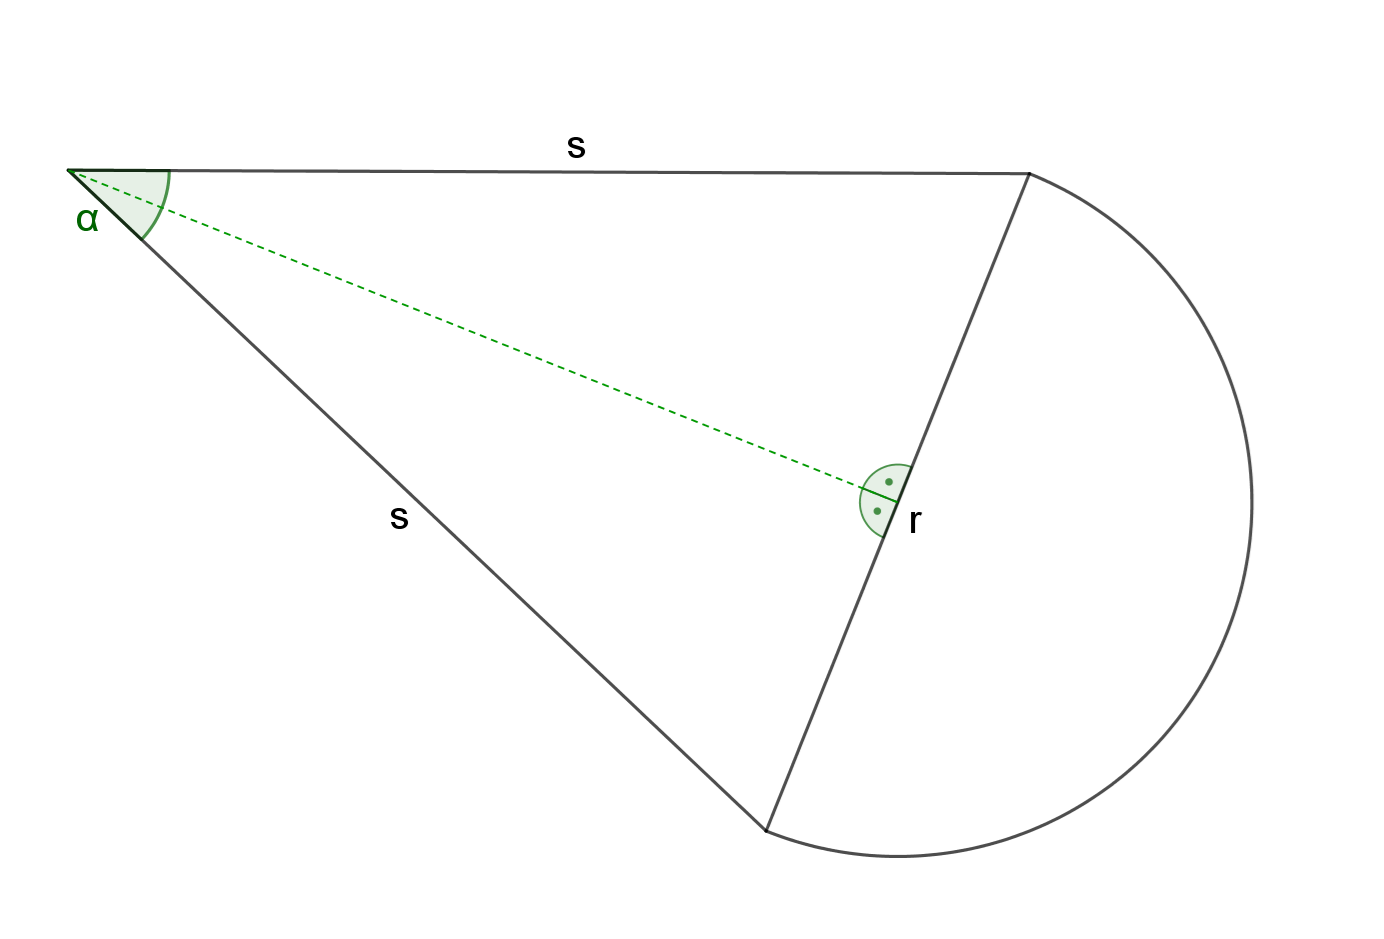
\includegraphics[width=0.6\textwidth]{figures/aufgabenstellung.png}
    \caption{Schematische Darstellung des Problems.}    
\end{figure}
